\documentclass[preprint]{sigplanconf}

\usepackage{amsmath}
\usepackage{color}
\usepackage{graphicx}
\usepackage[nice]{nicefrac}

%
% Macros and definitions:
%

%%% override thesis.cls's definitions for floats (figures):
\setcounter{topnumber}{2} % 1
\renewcommand*{\topfraction}{.9} % .4
\setcounter{totalnumber}{4} % 1?
\renewcommand*{\textfraction}{.07}
\renewcommand*{\floatpagefraction}{.7} % .3
%\setcounter{dbltopnumber}{1}
%\renewcommand*{\dbltopfraction}{.4}
%\renewcommand*{\dblfloatpagefraction}{.3}
\setlength{\abovecaptionskip}{5pt}  % 10pt
\setlength{\belowcaptionskip}{5pt} % 10pt


\def\Meta{Lorax}

\def\emp{\textit}  % thesis.cls changes \emph to bold, which sucks, so I define my own

\newcommand{\temp}[1]{ {\color{blue}#1} }

% font for literals in the presentation:
\newcommand{\keyword}[1]{\textbf{#1}}%{\ensuremath{\mathtt{#1}}}
\newcommand{\clojure}[1]{\texttt{#1}}%{\ensuremath{\mathtt{#1}}}

\def\lsyn{ {\color{blue}\left(\!\right.} }
\def\rsyn{ {\color{blue}\left.\!\right)} }

\newcommand{\todo}[1]{ {\textit{\color{red}[TODO: #1]}} }


%
% commands for reduction equations:
%
\newcommand{\mapnode}[2]{ {\mathbf{#1}~\{ #2 \}} }
\newcommand{\attr}[2]{ {\textit{#1} \mapsto #2} }


\newcommand{\seqnode}[2]{ {\mathbf{#1}~[ #2 ]} }

\newcommand{\reduces}{ \quad \longrightarrow \quad }

% \TeX seems to be built-in
%\def\tex{T\kern-.1667em\lower.5ex\hbox{E}\kern-.125emX\spacefactor1000}


% a way of setting off ???
%\newcommand{\syntax}[1]{\ensuremath{\fbox{\ensuremath{#1}}}}

% 
%\definecolor{literal}{rgb}{.8,.8,.6}
%\definecolor{literalbg}{rgb}{1,1,.8}

% deprecated:
%\newcommand{\embed}[1]{\ensuremath{\fcolorbox{literal}{literalbg}{\ensuremath{#1}}}}
%\newcommand{\unbed}[1]{\ensuremath{\fcolorbox{literal}{white}{\ensuremath{#1}}}}

%\newcommand{\quoted}[1]{\ensuremath{\fcolorbox{literal}{literalbg}{\ensuremath{#1}}}}
%\newcommand{\unquoted}[1]{\ensuremath{\fcolorbox{literal}{white}{\ensuremath{#1}}}}

%\newcommand{\node}[2]{\ensuremath{#1 \: \{ #2 \}}}
%\newcommand{\attr}[2]{\ensuremath{\mathrm{#1} : \: #2}}

%\newcommand{\reducep}{\ensuremath{\overset{present}{\longrightarrow}}}
%\newcommand{\reducec}{\ensuremath{\overset{compile}{\longrightarrow}}}

%\newcommand{\gray}[1]{ {\color[gray]{.7}#1}}
%\newcommand{\gparens}[1]{ \gray{(} #1 \gray{)} }

% formatting for selections:
%\definecolor{selection}{rgb}{1,.5,.8}


\begin{document}

\conferenceinfo{SIGPLAN WGP '11}{Sept. 9, 2011, Tokyo, Japan.} 
\copyrightyear{2011}
\copyrightdata{[to be supplied]} 

\titlebanner{banner above paper title (pre-print only)}        % These are ignored unless
\preprintfooter{short description of paper (pre-print only)}   % 'preprint' option specified.

\title{Bootstrapping a Language Workbench}
\subtitle{A Light-weight Approach to Language Oriented Programming}

\authorinfo{Moss Prescott and Jeremy Siek}
           {University of Colorado, Boulder}
           {\{moss.prescott,jeremy.siek\}@colorado.edu}

\maketitle

\begin{abstract}
% Shooting for ~200 words:
%Researchers and professionals in many fields are increasingly interested in defining new computer languages, but existing tools are not well-suited to this use. When popular general-purpose languages are extended, or when new text-based languages are created, the problem of parsing and the fundamental limits of text severely limit the form languages can take. On the other hand, a number of recent projects take a different approach wherein programs are stored in some sort of opaque tree structure. Instead of defining a parser, the language designer/user defines the abstract syntax 
\todo{Tried to start here but it was a disaster so instead worked on reducing the thesis to a compressed outline instead.}
\end{abstract}

\category{D.3.1}{Programming Languages}{Formal Definitions and Theory}  % ???

\terms
Languages, Syntax

\keywords
Syntax extension, Domain Specific Languages, Abstract syntax

\section{Introduction}

%\subsection{Role of Language Def. and Ext.}
Many kinds of programmers are interested in creating new computer languages, yet the technology that is most often used to construct new languages does not support creative activity well at all. Meanwhile, mature languages now come with very sophisticated editing tools\cite{eclipse}, but these tools require a large effort to create, and any new language therefore is at a major competitive disadvantage.

...another approach, often identified with the Lisp community, views the task of writing a program as combined with the building of a language into one activity \cite{on-lisp}...

Limitations of text as a vis. repr., and of parsers as a way of interacting with the compiler...

Promise and problems of structure editing as an approach...


\subsection{What a language's syntax can and should be}

Programs can look as good onscreen as they do in a paper or textbook...

When programs contain elements that have a familiar non-textual representation, they should be presented that way. Math, images, etc.

Take advantage of other forms of interaction besides character editing. 

Modern devices make all this possible. High res.~displays, sophisticated fonts, mice for cryin' out loud...


\subsection{Proposal and success criteria}

A new system for creating, transforming, and executing new languages, based on:

\begin{itemize}
\item AST as primary representation.
\item Transformation of ASTs.
\item Kernel language as target of reduction for execution, and as platform for implementing transformations.
\item Presentation language as a second target of reduction.
\end{itemize}

Goals:
\begin{itemize}
\item As easy to add elements as in LISP.
\item Presentation as good as published pseudo-code.
\item Editor can handle arbitrary language extension.
\item Modest implementation complexity.
\end{itemize}

\subsection{Roadmap}
Section 2 reviews the strengths and weaknesses of existing approaches. Section 3 presents a new approach based on ASTs from the ground up.
Section 4 shows examples of how the system works, using a prototype.
Section 5: related work. Section 6 concludes.


\section{Case Studies}
\label{studies}

To evaluate the success of \Meta\ at supporting the addition of new language constructs, I implemented two of them, using the grammar language to extend the \Meta\ core language. The first is a simple extension of the syntax for constructing lists (one of the basic data types of the core language), and the second introduces a completely new kind of value.

%
% Definition of 'for':
%
\subsection{Defining the Core Language via Syntax Extension}
\label{for}
The core language is built via syntax extension on top of the kernel language, so its definitions can serve as a test of the suitability of \Meta's \kw{grammar} facilities for building these kinds of extensions. This section compares one of the declarations from \Meta's core language with the corresponding elements from Lisp and free-form languages in terms the effort invested and the benefit accrued.

Several core language nodes provide support for using the primitive cons-list values of the Clojure platform, which are one of the basic tools for organizing data in any Lisp. These extensions employ a handful of Clojure primitives to expose the native list values of the platform, and the rest of the syntax is built around them.

%These definitions are typical of the kind of syntax extension which is used to build the elements of a language. In a Lisp, as in \Meta, this kind of syntax is reduced to the more primitive syntax of the kernel language (the special forms), whereas in a language with free-form syntax, these elements are typically built into the language's compiler. This section presents the declarations of a simple list comprehension syntax, and briefly compares the result with what would be necessary in the other approaches.

\subsubsection{List Comprehension in Lorax}

\begin{figure}[th]
	\centering
	
	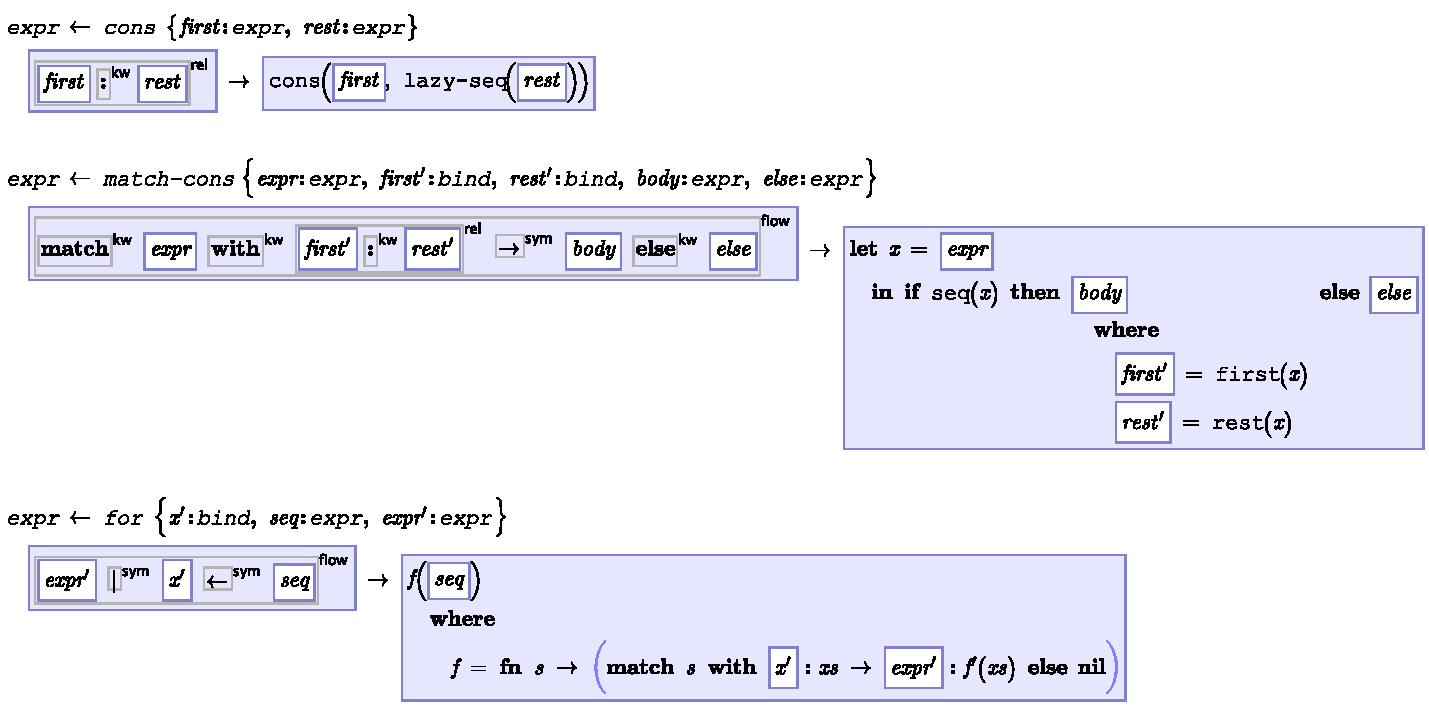
\includegraphics[scale=0.35]{src/image/cons.pdf}
	
	\caption{Declaration of the \kw{cons}, \kw{match-cons}, and \kw{for} node of the core language.}
	\label{fig-for-grammar}
\end{figure}

Figure \ref{fig-for-grammar} shows the declarations of the two primitive constructs for working with with lists (\kw{cons} and \kw{match-cons}), and a list comprehension (\kw{for}) node constructed from them. For the present purpose, the first two nodes can be regarded as part of the base language, and the list comprehension syntax as an extension to be added to that language.

%First is the constructor for lists: \kw{cons}. This node, displayed as a colon operator (as in Haskell), evaluates its \kw{first} child and uses Clojure's \cl{cons} function to construct a cons-cell with the resulting value as its head. \cl{lazy-seq} is applied to the \kw{rest} child, so that it is not evaluated until the value is needed. This introduces laziness into the core language (recall that the kernel language's semantics is entirely strict), allowing infinite lists to be constructed. Note: the application of \cl{lazy-seq} is translated by the meta-compiler to an application of the corresponding macro (with no special effort); if \cl{lazy-seq} was treated as an ordinary (strict) function application, some additional nodes would be required to wrap \kw{rest} in a lambda abstraction, say, to defer its evaluation.

%A \kw{match-cons} node de-constructs a list (see the second declaration in Figure~\ref{fig-for-grammar}). Its children consist of an expression (\kw{expr}) to be evaluated bindings for the head (\kw{first}) and the remainder (\kw{rest}) of the list, an expression (\kw{body}) to be evaluated if the match succeeds, and an alternative expression (\kw{else}) to be evaluated if the list is empty. The \emph{expand} reduction implements this by first binding the value of \kw{expr} to $x$ (a variable local to the reduction), then applying Clojure's \cl{seq} function, which tests whether the value represents a non-empty list. If so, the two bindings are bound to the parts of the cell using the corresponding Clojure primitive, and the \kw{body} expression is evaluated.

%These two nodes are all that is required to construct a variety of syntax for lists, none of which will need to use the lower-level primitives. The \kw{for} (list comprehension) node is also defined in Figure \ref{fig-for-grammar}. 
The \emph{expand} reduction for the \kw{for} node evaluates its \kw{seq} child, and then applies a recursive function to it. This function attempts to match its argument as a non-empty list (using \kw{match-cons}). If so, the \kw{x} child is bound to the first value, and \kw{expr} is evaluated and then the function is applied to the rest of the list. Note that one of the bindings (\kw{x}) was supplied by the programmer, and the other ($xs$) is local to the reduction. %Both \kw{x} and $xs$ are in scope when \kw{expr} is evaluated, thus in the new syntax, the binding introduced by \kw{x} is in scope in \kw{expr}, but not in \kw{seq}.

%The rest of the core language's syntax for working with lists is defined in a similar manner, using the \kw{cons} and \kw{match-cons} nodes, often in combination with a recursive function to traverse the list. Some examples of the resulting syntax are shown in Figure~\ref{fig-core}. Languages such as Haskell and Python provide such features as integral parts of their fixed grammar and compiler, but in \Meta\ equal or greater expressivity is achieved with a very small implementation effort and with complete modularity---any or all of these nodes can be removed or redefined by simply editing the grammar, without any impact on the rest of the language.

\subsubsection{List Comprehension in Lisp}

\begin{figure}[t]
\centering
\begin{verbatim}
=> (defmacro simple-for
     [[x xs] expr]
     `((fn f# [s#]
         (if (seq s#)
           (let [[~x & r#] s#]
             (cons ~expr
               (lazy-seq (f# r#))))))
         ~xs))

=> (simple-for [x (range 1 11)] (* x x))
(1 4 9 16 25 36 49 64 81 100)
\end{verbatim}

\caption{List comprehension macro in Clojure}
\label{fig-for-lisp}
\end{figure}

For comparison, the definition of a Clojure macro with equivalent capability is shown in Figure~\ref{fig-for-lisp}. The macro operates in a very similar way to the \Meta\ syntax declaration, so a fairly direct comparison of the two is revealing.

Both declarations make use of quasi-quoted syntax to construct a reduced program fragment. In \Meta, the rendering of quoted nodes using a contrasting background color provides a clear visual cue of the embedded structure. It's clear at a glance where the three components of the syntax are substituted into the reduced program. In Clojure, quotation and un-quotation are indicated with lexical signifiers (as in `\cl{`(\dots)}' and `\cl{\textasciitilde x}'), and it's up to the reader to count parentheses to understand what is evaluated when. To avoid unintended variable capture, names introduced in the Clojure reduction are marked with another signifier (as in `\cl{x\#}') which causes a new name to be generated each time the quotation is evaluated. In \Meta, no such signifiers are needed, because variable references are unambiguous---the meta-compiler takes care of generating new, unique labels when the quotation is expanded.

Thus the reduction/macro is of roughly equivalent complexity in the either system, but \Meta's handling of quotations and variable references makes the reduction both easier to read (via visual cues) and easier to write (by avoiding subtle issues of variable capture).

\subsubsection{Concrete Syntax}
In addition to this definition of semantics, \Meta's declaration defines a new syntax for the comprehension, which is designed to be familiar from both the mathematical notation of set theory and the comparable construct in Haskell. In \Meta, the reduction for this syntax is entirely trivial, simply giving the arrangement of the three child nodes and the symbols to be placed between them. The effort involved to provide such a simple reduction is essentially nil. For the programmer using the extended language, this syntax gives list comprehensions a distinct appearance. 

Returning to Clojure, the new syntax is limited to the few common elements used by all syntax in the language, with little more than the name ``simple-for'' distinguishing it from any other expression. A more illustrative comparison is with Haskell's similar construct. In Haskell, one can write the same example as follows:
\begin{verbatim}
[ x^2 | x <- [1..10] ]
\end{verbatim}
which has the same basic structure as the \Meta\ version, except that it suffers slightly for being limited to the ASCII character set.

However, Haskell's list comprehension syntax is baked into the compiler, and the programmer has no ability to add a new syntax of this kind without modifying the Haskell compiler's front-end. This is typical of languages with free-form syntax; what the language provides may work well, but the specification of syntax is inaccessible to the user (i.e.~it's outside the reach of what can be accomplished with a reasonable effort). \todo{Template Haskell? others?}

\subsubsection{Evaluation}
\Meta's facilities for declaring new syntax and specifying semantics and concrete syntax allow new syntax to be introduced with an effort that compares well to Lisp's macro facility. However, both the declaration of the new syntax and its use are significantly more readable than the corresponding Lisp programs, or even the syntax from Haskell which is designed for just this purpose. Meanwhile, the effort involved is much less than the effort would be to add such a construct to a language such as Haskell.


%
% Runtime (enumerating the rationals):
%
\subsection{Introducing a New Runtime Value}
The preceding section showed how the facilities of the platform can be exposed and wrapped in a novel syntax. This syntax helps the programmer to understand the program, but as soon as the program is reduced to the kernel language for evaluation, the syntax is gone and only the primitive values remain. A more ambitious goal for syntax extension is to augment the language with a new kind of runtime value. This allows programs to operate on a new kind of data, and allows the programmer to see results of computation in the natural form. The next example shows how a new kind of value can be introduced, and how it supports writing a program in a much more natural and comprehensible way.

\subsubsection{Enumerating the Positive Rationals}
In a delightful Functional Pearl \cite{gibbons}, Gibbons et al.\ present Haskell programs which generate the infinite series of all positive rational numbers. They begin with the idea of traversing the infinite matrix $a_{ij} = i/j$ which contains every positive ratio, but also contains many equivalent, unreduced ratios (e.g. $\nicefrac{1}{2}$, $\nicefrac{2}{4}$, $\dots$).

The authors show that a series containing all positive rationals in reduced form, without duplicates, is obtained by iterating the function 
$x' = 1/{(\lfloor x \rfloor + 1 - \{x\})},$\footnote{In the authors' notation, $\lfloor x \rfloor$ is the floor, or whole-number part of $x$, and $\{x\}$ is the fractional part: $\{x\} = x - \lfloor x \rfloor$, $x > 0$.} beginning with $x=1$. This is a surprisingly simple formula, but it is somewhat computationally undesirable in that calculating $\lfloor x \rfloor$ and $\{x\}$ involves division.

Interestingly, this formula can be implemented using only ``a constant number of arbitrary-precision integer additions and subtractions, but no divisions or multiplications'' by choosing a different representation for ratios. It happens that the five necessary operations---reciprocal, floor, addition of an integer, negate, and fractional part---can all be efficiently performed on ratios represented as \emph{regular continued fractions}. A continued fraction has the form\footnote{Incidentally, this expression is a frequently-cited exception to \TeX's rules for formatting fractions---all the nested expressions are best typeset at the same size, to emphasize the recursive structure. \Meta\ does not provide a way to override that behavior, so continued fractions do not look quite this nice in \Meta!}
$$a_0 + \frac{1}{
    \displaystyle a_1 + \frac{\displaystyle 1}{
        \displaystyle \cdots + \frac{\displaystyle 1}{
            \displaystyle a_n}}}$$
A regular continued fraction is one in which all the coefficients except $a_0$ are positive, and $a_n > 1$ (except for the special case 1). Every rational has a unique representation as a regular continued fraction.

Having arrived at this elegant result, the authors proceed to reduce their formulas to the notation of Haskell for implementation, using lists of integer coefficients to represent continued fractions. In the process, the origins of the code are completely obscured by the loss of the original notation. For example, one of four cases for negation of a regular continued fraction looks like this:\footnote{Actually, what's shown in the paper has been pretty-printed for publication \cite{lhs2tex}. In the actual source code, it must have looked something like this: \cl{negatecf [n\_0, 2] = [-n\_0-1, 2]}.}
%$$\mathit{negatecf} (n_0 : 1 : n_2 : ns) = (-n_0 - 1) : (n_2 + 1) : ns$$
%$$-\left(n_0 + \frac{1}{\displaystyle 1 + \frac{1}{n_2 + \cdots}}\right) = (-n_0 - 1) + \frac{1}{(n_2 + 1) + \cdots}$$
$$\mathit{negatecf}\:[n_0, 2] = [-n_0-1, 2]$$
It's up to the reader (of the paper or of the code) to decode the representation of fractions being used here and work out how this corresponds to the algebra that motivated it. However, in the proper notation, the same definition reads as simple algebraic equation which is easily understood and checked:
$$-\left(n_0 + \frac{1}{2}\right) = (-n_0 - 1) + \frac{1}{2}$$
The awkwardness of Haskell's notation is an impediment to understanding the program as an artifact, but it also obscures the program's meaning in a more subtle way. The choice of integer lists as a representation, as opposed to defining a new algrebraic data type with a similar recursive structure, was probably driven by the relative economy of the notation for lists (which is provided by the Haskell parser as a special case). As a result, accurate type information is lost, which makes the program harder to understand both in the writing and at runtime.

%\vspace{12pt}

\subsubsection{Continued Fractions in \Meta}
In \Meta, one can extend the language with a new kind of value for these fractions. I did this by defining a \kw{continuedFraction} node which defines a recursive data type. It is displayed in the obvious way, except that when the continuation is the ``null'' value, it is displayed in a slightly simplified form. The \emph{expand} reduction is new---it reduces to an expression which evaluates the component expressions and then constructs a node. Therefore the node itself becomes a runtime value. Several \kw{match} nodes provide pattern matching on the runtime shape of the argument, and are used to identify the cases in each operation. Figure~\ref{fig-cf} shows the declarations of the five operations. %, and some simple examples of their use are shown in Figure~\ref{fig-cfex}.
\begin{figure}[th]
  \centering
  
%  \todo{split into columns?}
  
  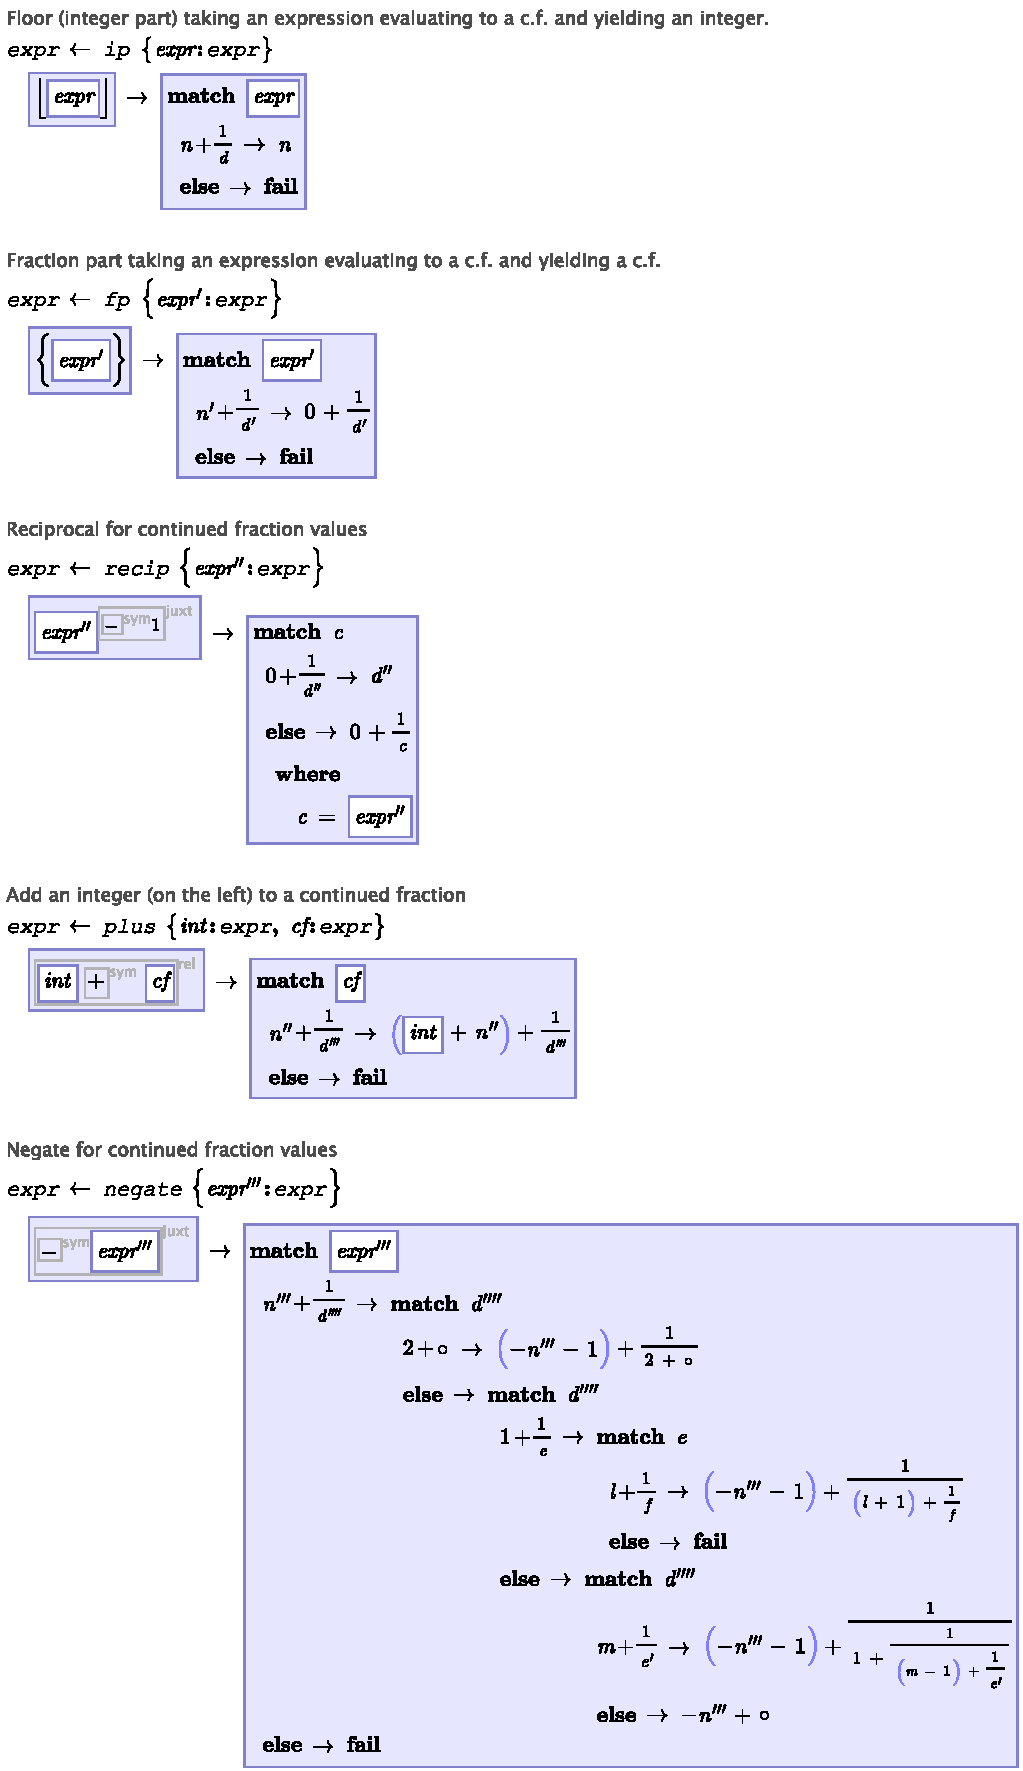
\includegraphics[scale=0.4]{src/image/continued-ops.pdf}
  
  \caption{Grammar for operations on continued fractions as runtime values.}
  \label{fig-cf}
\end{figure}

%\begin{figure}[th]
%  \begin{center}
%  
%  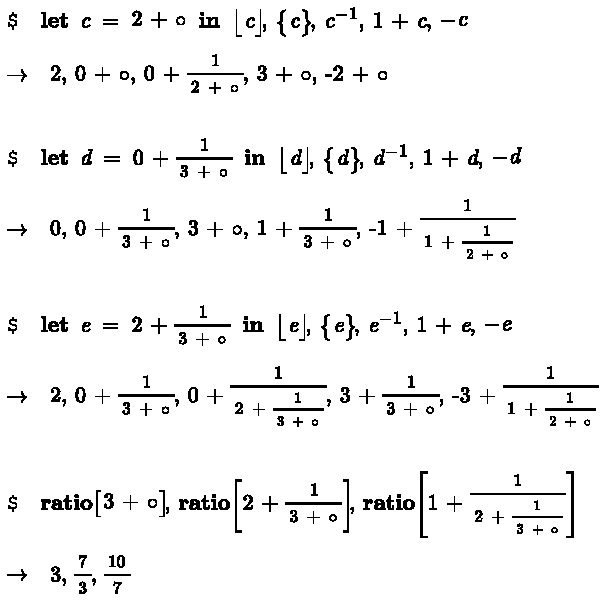
\includegraphics[scale=0.6]{src/image/continued.pdf}
%    
%  \end{center}
%  \caption{Operations on continued fractions.}
%  \label{fig-cfex}
%\end{figure}

%Note that these declarations are somewhat straining the current capabilities of \Meta. Ideally the construction of a runtime node would be as simple as adding a second level of quotation to the \kw{expand} reduction, but the current prototype does not handle that properly, so a bit of extra ceremony is required. In fact, in order to achieve the relatively understandable reductions shown in Figure~\ref{fig-cf}, I had to manually define a total of seven different \emph{match} nodes, out of a possible 16 for patterns up to three levels deep. It would be much more convenient to have a general pattern-match construct supporting multiple patterns, each a node with bindings substituted for some of the child nodes, but \Meta's current approach to reductions cannot handle that. Nevertheless, 
With the hard work of defining syntax and semantics out of the way, the actual algorithm can be expressed quite naturally. The expression which produces the next fraction in the series is wrapped in a function:
\begin{center}

\includegraphics[scale=0.8]{src/image/rationals-next.pdf}
\end{center}
Note that in this form the expression does not exactly match what was shown earlier, because some algebraic manipulation is necessary to put it into a form that uses only the operations that have been defined. The resulting expression contains one node (operator) for each operation to be performed. For instance, the original expression hid a negation and an addition operation behind a single $-$ symbol, but my version makes the two operations explicit. Also, \Meta\ inserts a pair of parentheses to clarify the order of evaluation of the two addition operations, another point which is left to algebraic convention in the original. Other than that, my choice of notation resembles the original precisely.

Now generating the infinite series in continued fraction form is as simple as applying the \emph{iterate} operator (${}^*$) to the $\mathit{next}$ function, using 1 as the initial value:
\begin{center}

\includegraphics[scale=0.8]{src/image/rationals-iter.pdf}
\end{center}
The complete expression and the first 15 fractions (converted to simple ratios) appear in Figure~\ref{fig-rationals}. 

% todo: more of a punchline?

\begin{figure}[t]
  \centering
    
  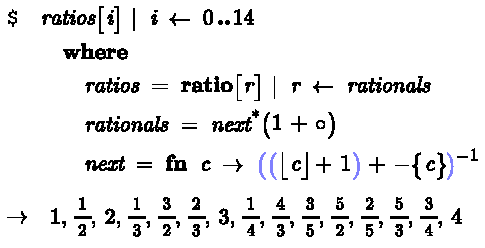
\includegraphics[scale=0.6]{src/image/rationals.pdf}
  
  \caption{Enumerating the rationals, using continued fractions.}
  \label{fig-rationals}
\end{figure}

\subsubsection{Evaluation}
\Meta\ allows a novel runtime value to be defined entirely in terms of nodes and reductions. Once a constructor and some syntax for pattern matching on the new values are defined, it's quite straightforward to implement operations on the new values, and to write programs which make use of the values and operations on them.

In the case of continued fractions, the notation is clearly superior to what can be done in a textual language, both aesthetically and in terms of ease of understanding. Furthermore, the improved notation encourages the use of a proper data type, as opposed to the awkwardness of Haskell which pushes the programmer towards using a generic data type to take advantage of a more convenient syntax.

One thing to note is the use of identical $+$ symbols for two distinct addition operations (first addition of integers, and then addition of an integer to a continued fraction). It might be preferable to use a different symbol for the new kind of addition. Because that symbol is specified in one place---the presentation reduction for that node---it's trivial to make the switch, without the need to update each use of the operator. On the other hand, this may be a case where some ambiguity in the visual representation can actually enhance readability. If that freedom leads to an incorrect program, it's easy to click on either node and the editor will indicate which $+$ is of which type. This represents a middle ground between the approach of ``overloading'' operators at the level of syntax, relying on the compiler or runtime to disambiguate them (as in C and many similar languages), and using a distinct operator for each type of argument (as in \todo{what's that language that uses \cl{.+} for adding FP numbers?}).

However, the current limitations of \Meta's approach to reductions make the job of defining these operations more arduous than it should be. A more general mechanism for implementing pattern-matching is needed to make this attractive.

%\subsection{Final Notes}
%Online syntax checking is a significant boon to developer productivity (as evidenced by the general adoption of syntax-highlighting editors and interactive-compiling IDEs), and \Meta\ provides much of the benefit of this technique through its simple grammar language. However there is one place where this checking is not effective: the contents of quoted nodes may have any type whatsoever, and an un-quote node must be allowed to appear anywhere at all. This is a consequence of the fact that \Meta\ grammars specify only local structure. For example, to properly constrain the nodes of a presentation reduction, it would be necessary to require that the value produced by the reduction is a node in the presentation language. As it is, this kind of error is not discovered until runtime (i.e. when the editor attempts to apply the reduction). And lacking this kind of information, the editor is not able to provide reasonable suggestions when editing quote nodes. This is a significant gap, but adding what amounts to a type system to \Meta\ for this purpose alone seemed ill-advised. Of course, many of the languages people want to use are statically typed, so a more complete system will probably need to solve that problem anyway.

%The most significant limitation of \Meta\ as a practical tool is its lack of integration with existing tools. The prototype editor could be developed into a stand-alone tool, and it could perhaps be used to generate traditional source or object code for use with another system. A more ambitious goal would be to integrate this style of editing into an existing IDE. Ultimately, many other integration points would need to be addressed, including most obviously source code management, but also any and all tools that aim to present or analyze source code.

\subsection{ASTs and Transformations}
[An open, general, persistent representation for trees; durable identity for all nodes; advantages thereof. ]

[Reductions and checkers \emph{based on attribute grammars}; attributes computed by functions in kernel language.]

\subsection{Transformations for Execution}
Introduce the kernel language, making it as little different from LC as poss.; handling of quotations. How a GPL is built from it.

\begin{figure}[ht]
	\begin{tabular}{ll}
	construct & concrete syntax
	\\
	\hline
	binding & $\kw{let}~x = e_1~\kw{in}~e_2$
	\\
	variable reference & $x$
	\\
	lambda abstraction & $\kw{fn}~x \rightarrow e$
	\\
	application (call-by-value) & $e_1(e_2)$
	\\
	conditional & $\kw{if}~e_1~\kw{then}~e_2~\kw{else}~e_3$
	\\
	special values & \kw{nil}, \kw{true}, \kw{false}
	\\
	literals (integers, strings, names) & 1, \textsf{abc}, \textit{foo}
	\\
	external reference & \texttt{cons}
	\\
	quotation & \todo{?}
	\\
	un-quotation & \todo{?}
	\\
	pattern-matching & $\kw{match}~e_1~\kw{with}~p \rightarrow e_2~\kw{else}~e_3$
	\end{tabular}

	\caption{A kernel meta-language}
	\label{fig-kernel}
\end{figure}

Figure~\ref{fig-kernel} shows...


\subsection{Transformations for Presentation}
Brief description of the high-level presentation AST; how source is reduced to it; how it supports easy extension and modularity. Very brief mention of how it actually gets rendered [via a further reduction to a low-level language, via attributes].

\subsection{A few details}
Tracking of source nodes; parenthesization (just an example, without harping on it).


\section{Lorax 0.2}
\label{lorax}
To build programs directly out of nodes, we need a common representation for nodes. It must be flexible enough to represent many kinds of programs and support the kind of editing operations we will want to provide. It should provide a natural way to represent the primitive values which appear in programs, and the common ways of aggregating values into larger structures. It should be able to represent arbitrary programs, and allow nodes to be freely composed without imposing any fixed constraints.

Also, AST nodes will be called on to represent elements of not only source programs, but also intermediate programs, grammars, and graphical elements.

\subsection{Nodes, Values, and References}
A \emph{program} is a tree made up of \emph{nodes}. Every node has a \emph{type}, a unique \emph{label}, and a \emph{value}. A node's type identifies it as one of a class of related nodes, all of which have some common meaning (for example, the type \kw{plus} might represent addition expressions). A node's label is an opaque identifier which gives it a distinct identity, and allows references to nodes to survive transformations of the program. A node's value may be: \emph{empty}, if the node type alone carries all the node's meaning; an atomic value, which is a \emph{boolean}, \emph{integer}, or \emph{string} (a sequence of characters which are treated as an indivisible value); a \emph{sequence} of $n$ child nodes (indexed by integers $0$ to $n-1$) or an (unordered) \emph{map} of distinct \emph{attribute names} and associated child nodes. A \emph{reference} is a special type of node which has the type \kw{ref}, and has as its value the label of another node.

We define these four kinds of nodes because they seem to be sufficient to represent the elements of programs for the languages we experimented with. These elements seem to fall into four categories, corresponding to the four kinds of nodes. Of the four, map nodes are the most commonly used, and their ability to contain an arbitrary set of attributes is key to the extensibility of the system. Sequences are represented with a first-class node type primarily for the convenience of the editor, discussed later. Reference nodes represent any reference from one part of a program to an entity which is declared elsewhere, rendering such references unambiguous.

Nodes are immutable values, so a program is a \emph{persistent data structure} \cite{sarnak}. A modified program may be constructed by building a new tree sharing much of the structure of an existing tree, which allows an efficient system to be built out of many layers of tree transformation.

A program is \emph{well-formed} if its nodes satisfy the following constraints:
\begin{enumerate}
\item No two nodes have the same label.
\item No node appears as a child of more than one parent, or under more than one index/name of a sequence/map-valued node (i.e. the nodes form a tree).
\item The value of each reference node is the label of some node in the program.
\end{enumerate}

Note that any node can be considered as the root node of a sub-tree consisting of its descendant nodes. A sub-tree of a well-formed tree will be well-formed unless it contains a reference to a node which is not part of the same sub-tree. Such a reference is analogous to a free variable, and can play a similar role.

These minimal constraints allow trees to be transformed into one another using familiar functional programming techniques, and ensure that operations on trees have well-defined results. Therefore, \Meta\ requires that trees be well-formed at all times, and its components are designed to enforce these constraints.


\subsection{Specifications}
A \emph{specification} constrains the structure of nodes in a program. A program is \emph{valid} with respect to a certain specification if the arrangement of nodes, values, and references satisfies the specification's constraints.

In practice a program may contain violations of a specification, and the user will be interested in the nature of each violation in order to be able to fix them (by correcting either the program or the specification). Therefore a specification will typically be implemented in the form of a \emph{checker}, a function over programs that produces a set of \emph{errors} each consisting of a description of the problem and the location where it occurs.

Depending on the nature of the properties being checked, a specification may be defined only in terms of \emph{local} properties of individual nodes and their direct children, or may refer to \emph{non-local} relationships between nodes more distantly connected. In general, local properties are easier to define, easier to check, and easier to understand, so for the most part they are to be preferred. In section \ref{grammars}, we describe a particularly direct and convenient way of specifying these basic structural properties which is sufficient to define the abstract syntax of a programming language.

By providing a modular way of describing and checking properties of programs, specifications give much-needed structure to the open model of ASTs described in the preceding sections. They do not, however, restrict the user's ability to modify and extend her program and/or language, even if that means the program is invalid at times.


\subsection{Reductions}
\label{reduction}
The next step in making a useful system is providing a way to produce (multiple) \emph{target} programs from a given \emph{source} program. The central idea is to have a source program, consisting of nodes in some ``user'' programming language, which includes a node type for every important programming construct. In an extensible system, the user is able to add new types of nodes or even entire languages to a running system, even though the underlying system only understands a fixed set of node types. The way to bridge this gap is via \emph{reduction}.

Reduction is a restricted form of \emph{graph reduction}, inspired by the macro expansion process of Lisp.\footnote{The term ``Lisp'' is meant to refer to any of the many variants of Lisp, including Maclisp, Common Lisp, Emacs Lisp and Scheme.} In fact the term ``expansion'' might be more appropriate because a typical reduction replaces a more abstract node with a larger number of simpler nodes.

A \emph{source} program is reduced to a \emph{target} program by applying a \emph{reduction function} to the root node of the source program. If any reduction is possible, the reduction function returns a new, replacement root node, which typically repackages the children of the original root node under some new kind of parent. As long as some reduction is performed, the reduction function is applied repeatedly to the previous result. Eventually, the root node is fully-reduced (the function fails to return a new reduced node). At that point, each child node is reduced in the same way, and a new root node is constructed with the reduced children.

%Because each reduction step constructs an arbitrary replacement node, it's possible at least in theory to write any arbitrary transformation as a reduction. This means, for one thing, that reduction may not terminate. This generality, and the potential errors it allows, are typical of meta-programming systems; the full power of the language is available at compile-time, including the ability to introduce bad behavior. Although a system with less expressive power might be capable of meeting the need with less potential for bad behavior, in practice the kinds of problems that are encountered are most often easily fixed, provided that the system gives reasonably good error reports and no permanent damage is done when reductions do not perform as expected.

%During reduction a series of intermediate programs are produced which are partially reduced, and in general do not conform to the source or target specification. It might be interesting to investigate ways of defining specifications and reductions such that it could be statically shown that a valid source program always reduces to a valid target program. I have not investigated how this might work, but it certainly would require imposing restrictions on the results that could be produced by reductions, suggesting at the very least a static type system for the language of reductions.

%As a practical matter, it's convenient to define reduction functions only for properly-formed inputs. This can be facilitated by declaring both the specification (e.g. expected attributes for each node type) and the reduction (given a node with those attributes) at the same time. If the specification defines only local properties, then the reduction should assume only the presence of \emph{some} node at each required location, but make no demands on the form of these child nodes. 



%\subsection{Passing information down}
%A local reduction works by examining one node at a time, producing a reduced node which combines the children of the original node in a new way, possibly with some additional nodes inserted as well. This is often sufficient, but in some cases it's necessary to propagate some additional information through the reduction process. A simple extension that meets many needs is to augment the reduction function described above to accept an additional \emph{environment} parameter, an arbitrary value, and to return both a reduced node and a new environment value. When recursively visiting child nodes, the value resulting from the parent's reduction is used. This allows the reduction function to compute values based on the shape of the tree and use them to control some aspects of the reduction. For example, a reduction could keep track of the depth of the tree (distance from the root node).

%This simple approach works because the children of each node are always available to the reduction function, while the parent nodes are not. The ``inherited'' value allows the reduction function to accumulate some information about the otherwise inaccessible ancestors.

\subsection{Defining Specifications and Reductions}

\todo{A place to talk about defining transformations via attribute grammars and meta-language.}


\subsection{Characteristics}
This way of constructing program source has some implications for the way languages can be defined and the way programs can be worked with.

Node types, attributes, and specifications naturally fit with the concepts of \emph{tree grammars}, which allows specifications to be defined in ways that are familiar to language designers (i.e. with a grammar). Because grammars so-defined will be used only for checking tree structure and not for parsing, they can be constructed in the natural way, without any need for tricks to work around parsing algorithm shortcomings (e.g. left-factoring).

Programs are \emph{self-describing}. Each node carries an explicit declaration of its meaning, and each primitive value is manifestly of a certain type. This is in contrast to a textual language, where the same sequence of characters might represent a name, data, or a keyword, depending on the context in which they appear. This is a major advantage especially for tools that manipulate programs, because no parser is necessary to extract the structure of the program.

Labels provide robust \emph{source locations}. The label provides each node with an identity that survives when the other parts of the program are changed, or when the program is serialized to non-volatile storage, etc. Thus labels provide a way for tools (e.g. compilers and debuggers) to refer to source locations. For example, a typical refactoring operation such as changing the name of a variable or moving some code from one place to another looks like several unrelated changes to a \emph{diff} tool that has two versions of source text to look at, but a similar tool operating on labeled nodes could compare each \emph{node}, even if the location, the content, and even the type of the node have changed.

Reference nodes provide a way of referring to entities in a program which can never be ambiguous, and is independent of such language-specific notions as names and scope. Reference nodes require special support from editors, which may also take advantage of the explicit reference structure to provide enhanced presentation of references.

Programs may be serialized for storage, distributed processing, etc. For example, assuming a choice of character set and encoding, all the components of a node can be easily converted to a stream of characters. Because the representation permits only trees, each node can be serialized when it first occurs; there's no need for an encoding of back-references. Moreover, the choice of serialized format is not so important because the structure of programs is defined at the level of nodes. Any serialized form that preserves the meaning in the terms defined above is equally good.

\todo{Cut the rest of this section?} This representation of programs as nodes has some things in common with a handful of other tree-structured representations often used for source code and/or intermediate representations within tools such as compilers.

\subsubsection{Compared to XML}
XML and other related \emph{markup languages}, are designed to augment textual data with explicit structure for a variety of purposes. The structure of an XML document has much in common with the structure of nodes as defined here, and the \emph{XML Infoset}\cite{infoset} model for documents in particular has a similar flavor. However, there are some important differences:
\begin{enumerate}
\item The child elements of each node in an XML document are always in an ordered sequence, while named attributes can contain only simple character data. In \Meta, a node's children may be ordered or named, whichever makes sense, and there is no separate notion of attribute values vs. child nodes.
\item XML is explicitly a format for character streams, onto which an abstract model can be imposed \textit{post-hoc}. This leads to many awkward and ultimately uninteresting problems, such as when to ignore white-space and when it should be included in the data model. In \Meta, the source AST is defined in terms of the relevant types, and only nodes that actually contain character data are represented as characters.
\item Because XML is meant to be human-readable in a weak sense, text-editors are still the dominant mode of interaction with it. Although there are WYSIWYG tools for editing and viewing certain kinds of XML documents (e.g. SVG\cite{svg}, docx\cite{openoffice}), there are few general-purpose tools for working with XML per se, aside from text editors.
\end{enumerate}

XML's undesirability as a concrete syntax for programs has been well-established, and stands as an example of the usability challenges posed by representing source code as structured data \cite{holub}\cite{xml-bad-ant}. I believe this this failure largely results from the use of the textual representation as the editing interface. Although the XML syntax is particularly bad in this regard, any general-purpose, textual markup language will suffer in terms of readability for the flexibility it provides.

\subsubsection{Compared to S-expressions}
Most Lisp programs are written in \emph{s-expressions}, a simple data structure offering only lists, symbols (i.e. names), and a handful of types of primitive values. This simplicity gives considerable generality and flexibility, because it allows any number of new constructs to be introduced simply by defining new forms (macros). However, the use of s-expressions directly in lieu of a concrete syntax has been a highly divisive choice, essentially separating the population of programmers into two ``camps''. Only those who are not put off by sequences of nested parentheses can appreciate the expressive power that Lisp offers.

It is a major goal of this thesis to establish that the expressive power of the Lisp model can be realized in the context of a language that can be read by ``the rest of us.'' \Meta's representation for nodes has the same generality and free extensibility as s-expressions, and its simple and unambiguous structure makes it ideal for defining and transforming programs.

%\subsection{Compared to Algebraic Data Types}
%When language tools are written in functional languages such as Haskell and ML, nodes are often represented using \emph{algebraic data types}\cite{functionalAST}. Algebraic data types are rarely used directly to represent programs (because they are even more syntactically awkward than s-expressions), but are often used to represent programs after parsing. 

%The major difference is that these values are constrained by the type system to be valid. \Meta's nodes are subject to fewer hard restrictions, which allows programs to be freely modified by the programmer in the process of constructing and modifying the program.


\section{Expression Language}
\label{expr}

A new language for displaying programs, mathematical expressions, and simple graphical elements.

Nodes represent visual elements at a fairly abstract level. Source program is reduced to expression language.

From \TeX: algorithms, symbols, inspiration.

Space is part of the language. Parentheses are inserted as needed by a generic transformation (no need for language designer or user to worry about it).



\section{Evaluation}
\label{eval}

Experience with the prototype system allows some comparison to be made with existing systems.

\begin{table}
	\centering
	
	\begin{tabular}{lcc}
	 & Lorax LOC & MPS LOC
%	\hline
	\\
	foo & 100 & 10,000
	\end{tabular}
	
	\caption{Comparison of estimated lines of code...}
	\label{table-loc}
\end{table}

Table~\ref{table-loc} ...

\section{Related Work}
\label{related}
[Not the language workbenches, but other AST-based work?]

\section{Conclusion}
\label{conclusion}
~

%\appendix
%\section{Appendix Title}

%This is the text of the appendix, if you need one.

%\acks

%Acknowledgments, if needed.

% We recommend abbrvnat bibliography style.

%\bibliographystyle{abbrvnat}
\bibliographystyle{plain}

% The bibliography should be embedded for final submission.
\bibliography{src/refs}

%\begin{thebibliography}{}
%\softraggedright

%\bibitem[Smith et~al.(2009)Smith, Jones]{smith02}
%P. Q. Smith, and X. Y. Jones. ...reference text...

%\end{thebibliography}

\end{document}
